\documentclass[runningheads]{llncs}
\usepackage{graphicx}
%\usepackage[UKenglish]{babel}
%\usepackage[UKenglish]{isodate}
%\usepackage[utf8]{inputenc}
\usepackage[ruled,vlined]{algorithm2e}
\usepackage{amssymb}
\usepackage{mathtools}
\usepackage[capitalise]{cleveref}
\usepackage{tikz}
\usepackage{mathrsfs}

\newtheorem{constraint}{Constraint}

\newcommand{\variable}[1]{\texttt{\textup{#1}}}
\newcommand{\arrayd}[3]{\variable{{#1}[}{#2}\variable{]} \in {#3}}
\newcommand{\arrayt}[3]{\variable{{#3}[}{#2}\variable{] {#1}}}
\newcommand{\predicates}{\mathcal{P}}
\newcommand{\variables}{\mathcal{V}}
\newcommand{\constants}{\mathcal{C}}
\newcommand{\tokens}{\mathcal{T}}
\newcommand{\arities}{\mathcal{A}}
\newcommand{\maxArity}{\mathcal{M}_{\mathcal{A}}}
\newcommand{\maxNumNodes}{\mathcal{M}_{\mathcal{N}}}
\newcommand{\maxNumClauses}{\mathcal{M}_{\mathcal{C}}}

%\relpenalty=10000
%\binoppenalty=10000
\def\multiset#1#2{\ensuremath{\left(\kern-.3em\left(\genfrac{}{}{0pt}{}{#1}{#2}\right)\kern-.3em\right)}}

\begin{document}

\title{Generating Random Logic Programs Using Constraint Programming}
\author{Paulius Dilkas\orcidID{0000-1111-2222-3333}}
\authorrunning{P. Dilkas}
% First names are abbreviated in the running head.
% If there are more than two authors, 'et al.' is used.

\institute{University of Edinburgh, Edinburgh, United Kingdom\\
  \email{p.dilkas@sms.ed.ac.uk}}
\maketitle

\begin{abstract}
The abstract should briefly summarize the contents of the paper in
150--250 words.

\keywords{Constraint Programming \and Logic Programming \and Probabilistic Logic
  Programming.}
\end{abstract}

\section{Introduction}

Motivation:
\begin{itemize}
\item Generating random programs that generate random data.
  %For example, enforcing that the decision is independent of gender.
\item Learning: how this can be used for (targeted) learning, when (atomic)
  probabilities can be assigned based on counting and we can have extra
  constraints. A more primitive angle: generate structures, learn weights.
\end{itemize}

We will often use $\Box$ as a special domain value to indicate some kind of
exception. We write $\arrayd{a}{b}{c}$ to mean that
$\variable{a}$ is an array of variables of length $b$ such that each element of
$\variable{a}$ has domain $c$. Similarly, we write $\arrayt{a}{b}{c}$ to denote
an array $\variable{a}$ of length $b$ such that each element of $\variable{a}$
has type $\variable{c}$. All constraint variables in the model are integer
variables, but, e.g., if the integer $i$ refers to a logical variable $X$, we
will use $i$ and $X$ interchangeably. All indices start at zero.

We also use Choco~4.10.2 \cite{choco}. This works with both Prolog
\cite{DBLP:books/daglib/0041598} and ProbLog \cite{DBLP:conf/ijcai/RaedtKT07}.
Tested with SWI-Prolog \cite{DBLP:journals/tplp/WielemakerSTL12}.

\subsection{TODO}

\begin{itemize}
\item A constraint for logical equivalence. An algorithm to reduce each tree to
  some kind of normal form. Not doing this on purpose. Leaving for further work.
\item Perhaps negative cycle detection could use the same graph as the
  independence propagator? If we extend each domain to {-1, 0, 1}, but that
  might make propagation weaker or slower.
\item Could investigate how uniform the generated distribution of programs is.
  Distributions of individual parameters will often favour larger values
  because, e.g., there are more 5-tuples than 4-tuples.
\item Inference options to explore. Logspace vs normal space. Symbolic vs
  non-symbolic. Propagate evidence (might be irrelevant)? Propagate weights?
  Supported knowledge compilation techniques: sdd, sddx, bdd, nnf, ddnnf, kbest,
  fsdd, fbdd.
\item Mention the random heuristic. Mention that restarting gives better
  randomness, but duplicates become possible. Restarting after each run is
  expensive. Periodic restarts could be an option.
\end{itemize}

\subsection{Parameters}

Parameters:
\begin{itemize}
\item a list of predicates $\predicates{}$,
\item a list of their arities $\arities{}$ (including zero),
  \begin{itemize}
  \item maximum arity $\maxArity{} \coloneqq \max \arities{}$.
  \end{itemize}
\item a list of variables $\variables{}$,
\item and a list of constants $\constants{}$.
  \begin{itemize}
  \item Each of them can be empty, but $|\constants{}| + |\variables{}| > 0$.
  \end{itemize}
\item a list of probabilities that are randomly assigned to clauses,
\item option to forbid all cycles or just negative cycles,
\item $\maxNumNodes{} \ge 1$: maximum number of nodes in the tree representation
  of a clause,
\item $\maxNumClauses{} \ge |\predicates{}|$: maximum number of clauses in a
  program,
\item maximum number of solutions,
\end{itemize}

We also define $\tokens{} = \{ \neg, \land, \lor, \top \}$. All decision
variables of the model are contained in two arrays:
\begin{itemize}
\item $\arrayt{bodiesOfClauses}{\maxNumClauses{}}{Body}$,
\item $\arrayt{headsOfClauses}{\maxNumClauses{}}{Head}$
\end{itemize}

\section{Heads of Clauses}
% TODO: section for clauses. define heads & bodies, then separate subsections
% for head and body constraints

Our definition is slightly more involved because we want to eliminate some
symmetries.

\begin{definition}
  The \emph{head} of a clause is composed of:
  \begin{itemize}
  \item a $\variable{predicate} \in \predicates \cup \{ \Box \}$.
  \item and $\arrayd{arguments}{\maxArity{}}{\constants{} \cup \variables{}}
    \cup \{ \Box \}$
  \end{itemize}
  In both cases, $\Box$ is the disabled value.
\end{definition}

\begin{definition}
  The \variable{predicate}'s $\variable{arity} \in [0, \maxArity{}]$ can then be
  defined using the \variable{table} constraint as
  \[
    \variable{arity} = \begin{cases}
      0 & \text{if } \variable{predicate} = \Box\\
      \text{the arity of } \variable{predicate} & \text{otherwise.}
    \end{cases}
  \]
\end{definition}

\begin{constraint}
  For $i = 0, \dots, \maxArity{} - 1$,
  \[
    \variable{arguments}[i] = \Box \iff i \ge \variable{arity}.
  \]
\end{constraint}

\section{Bodies of Clauses}

\begin{definition}
  The body of a clause is defined by:
  \begin{itemize}
  \item $\arrayd{treeStructure}{\maxNumNodes{}}{[0, \maxNumNodes{} - 1]}$ such
    that:
    \begin{itemize}
    \item $\variable{treeStructure}[i] = i$: the $i$-th node is a root.
    \item $\variable{treeStructure}[i] = j$: the $i$-th node's parent is node $j$.
    \end{itemize}
  \item $\arrayt{treeValues}{\maxNumNodes{}}{Node}$.
  \end{itemize}
\end{definition}

Auxiliary variables: $\variable{numNodes}, \variable{numTrees} \in \{ 1, \dots,
\maxNumNodes{} \}$. The former counts the number of nodes in the main tree. The
latter counts the number of trees in total.

\begin{figure}[t]
  \centering
  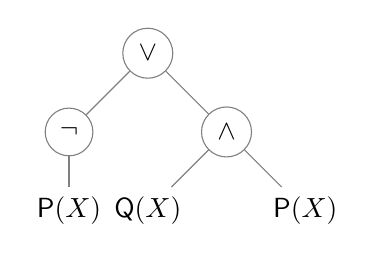
\begin{tikzpicture}
    \node[draw,circle,gray,text=black] (or) at (0, 0) {$\lor$};
    \node[draw,circle,gray,text=black] (not) at (-1, -1) {$\neg$};
    \node (P) at (-1, -2) {$\mathsf{P}(X)$};
    \node[draw,circle,gray,text=black] (and) at (1, -1) {$\land$};
    \node (Q) at (0, -2) {$\mathsf{Q}(X)$};
    \node (R) at (2, -2) {$\mathsf{P}(X)$};
    \draw[gray] (or) -- (not);
    \draw[gray] (or) -- (and);
    \draw[gray] (not) -- (P);
    \draw[gray] (and) -- (Q);
    \draw[gray] (and) -- (R);
  \end{tikzpicture}
  \caption{A tree representation of the formula from \cref{example:formula}}
  \label{fig:example_tree}
\end{figure}

\begin{example} \label{example:formula}
  Let $\maxNumNodes{} = 8$. Then $\neg\mathsf{P}(X) \lor (\mathsf{Q}(X)
  \land \mathsf{P}(X))$ corresponds to the tree in \cref{fig:example_tree} and
  can be encoded as:
  \begin{alignat*}{8}
    \variable{treeStructure} &= [0, &&0, &&0, &&1, &&2, &&2, &&6, &&7],\\
    \variable{treeValues} &= [{\lor}, &&{\neg}, &&{\land}, \mathsf{P}(&&X), \mathsf{Q}(&&X), \mathsf{P}(&&X), &&\top, &&\top],\\
    \variable{numNodes} &= 6, && && && && && && &&\\
    \variable{numTrees} &= 3. && && && && && && &&
  \end{alignat*}
  In the rest of this section, we will describe how the elements of
  $\variable{treeValues}$ are encoded and list a series of constraints that make
  this representation unique.
\end{example}

\subsection{Nodes}

\begin{definition} \label{def:node}
  A \emph{node} has a $\variable{name} \in \tokens{} \cup \predicates{}$ and
  $\arrayd{arguments}{\maxArity{}}{\variables{} \cup \constants{} \cup \{ \Box
    \}}$, where $\Box$ denotes a disabled argument (the reason why this value is
  needed will become clear in \cref{sec:variable_symmetry}). The node's
  $\variable{arity} \in [0, \maxArity{}]$ is defined by a \variable{table}
  constraint as
  \[
    \variable{arity} = \begin{cases}
      \text{the arity of } \variable{name} & \text{if } \variable{name} \in
      \predicates{}\\
      0 & \text{otherwise.}
    \end{cases}
  \]
\end{definition}

\begin{constraint}
  For $i = 0, \dots, \maxArity{} - 1$,
  \[
  \variable{arguments}[i] = \Box \quad \iff \quad i \ge \variable{arity}.
  \]
\end{constraint}
% TODO: this could merged into a single constraint for termsPerClause

\begin{example}
  Let $\maxArity{} = 2$, $\predicates{} = [\mathsf{P}, \dots]$, $\arities{}
  = [1, \dots]$, and $X \in \variables{}$. Then the node representing atom
  $\mathsf{P}(X)$ has:
  \begin{align*}
    \variable{name} &= \mathsf{P},\\
    \variable{arguments} &= [X, \Box],\\
    \variable{arity} &= 1.
  \end{align*}
\end{example}

\subsection{Constraints}

\begin{constraint}
  \variable{treeStructure} represents \variable{numTrees} trees, i.e.,
  \[
    \variable{tree}(\variable{treeStructure}, \variable{numTrees})\footnote{This
      constraint uses dominator-based filtering by Fages and Lorca
      \cite{DBLP:conf/cp/FagesL11}.}.
  \]
\end{constraint}

\begin{constraint}
  $\variable{treeStructure}[0] = 0$.
\end{constraint}

\begin{constraint}
  $\variable{numTrees} + \variable{numNodes} = \maxNumNodes{} + 1$.
\end{constraint}

\begin{constraint}
  \variable{treeStructure} is sorted.
\end{constraint}

\begin{constraint}
  For $i = 0, \dots, \maxNumNodes{} - 1$, if $\variable{numNodes} \le
  i$, then
  \[
    \variable{treeStructure}[i] = i \quad \text{and} \quad
    \variable{treeValues}[i].\variable{name} = \top,
  \]
  else
  \[
    \variable{treeStructure}[i] < \variable{numNodes}.
  \]
\end{constraint}

\begin{constraint}
  For $i = 0, \dots, \maxNumNodes{} - 1$,
  \begin{align*}
    \variable{count}(i, \variable{treeStructure}_{-i}) = 0 &\iff \variable{treeValues}[i].\variable{name} \in \predicates{} \cup \{ \top \},\\
    \variable{count}(i, \variable{treeStructure}_{-i}) = 1 &\iff \variable{treeValues}[i].\variable{name} = \neg,\\
    \variable{count}(i, \variable{treeStructure}_{-i}) > 1 &\iff \variable{treeValues}[i].\variable{name} \in \{ \land, \lor \}.
  \end{align*}
  $\variable{treeStructure}_{-i}$ denotes array $\variable{treeStructure}$ with
  position $i$ skipped.
\end{constraint}
Each constraint corresponds to node $i$ having no children, one child, and
multiple children, respectively.


\begin{constraint}
  For $i = 0, \dots, \maxNumNodes{} - 1$,
  \[
    \variable{treeStructure}[i] \ne i \implies
    \variable{treeValues}[i].\variable{name} \ne \top.
  \]
\end{constraint}

\begin{constraint}
  For $i = 0, \dots, \maxNumClauses{} - 1$, if
  $\variable{headsOfClauses}[i].\variable{predicate} = \Box$, then
  \[
    \variable{bodiesOfClauses}[i].\variable{numNodes} = 1,
  \]
  and
  \[
    \variable{bodiesOfClauses}[i].\variable{treeValues}[0].\variable{name} =
    \top.
  \]
\end{constraint}

\section{Eliminating Variable Symmetries} \label{sec:variable_symmetry}

Given any clause, we can permute the variables in it without changing the
meaning of the clause or the entire program. Thus, we want to fix an order on
variables to eliminate unnecessary symmetries. Informally, we can say that
variable $X$ goes before variable $Y$ if its first occurrence in either the head
or the body of the clause is before the first occurrence of $Y$.

\begin{definition}
  Head:

  size: $|\constants{}| + |\variables{}|$

  domain: $\{ 0, \dots, \maxArity{} - 1\}$

  condition: for $i = 0, \dots, \maxArity{} - 1$ and $t \in \constants{} \cup \variables{}$,
  \[
    \variable{arguments}[i] = t \quad \iff \quad i \in \variable{occurrences}[t].
  \]

  Body:

  size: $|\constants{}| + |\variables{}| + 1$

  domain: $\maxNumNodes{} \times \maxArity{}$

  condition: for $i = 0, \dots, \maxNumNodes{} - 1$, $j = 0, \dots, \maxArity{}
  - 1$, $t \in \constants{} \cup \variables{} \cup \{ \Box \}$,
  \[
    \variable{treeValues}[i].\variable{arguments}[j] = t \quad \iff \quad i
    \times \maxNumNodes{} + j \in \variable{occurrences}[t]
  \]

  We define an array \variable{occurrences} of  sets such that, for all $t \in
  \constants{} \cup \variables{}$, $\variable{occurrences}[t]$ is a subset of
  that stores the indices of \variable{arguments} at which $t$ is located. It is
  defined by the \variable{setsIntsChanneling} constraint equivalent to the
  following condition:
\end{definition}

\begin{definition}
  We define a $|\variables{}| \times 2$ matrix $\mathbf{M}$ with domain $[0,
  \maxNumNodes{} \times \maxArity{}]$ such that for $v = 0, \dots, |\variables{}| - 1$,
  \begin{align*}
    M_{v,0} &= |\variable{occurrences}[v]|.\\
    M_{v,1} &= \begin{cases}
      \min \variable{occurrences}[v] & \text{if } \variable{occurrences}[v] \ne \emptyset\\
      \maxNumNodes{} \times \maxArity{} & \text{otherwise.}
    \end{cases}
  \end{align*}
\end{definition}

\begin{constraint}
  We can then impose the \variable{lexChainLessEq} constraint on $\mathbf{M}$
  which means that for $v = 1, \dots, |\variables{}| - 1$,
  \[
    |\variable{occurrences}[v - 1]| \le |\variable{occurrences}[v]|,
  \]
  and if $|\variable{occurrences}[v - 1]| = |\variable{occurrences}[v]| > 0$,
  then
  \[
    \min \variable{occurrences}[v - 1] \le \min \variable{occurrences}[v].
  \]
\end{constraint}

\begin{example}
  Let $\maxArity{} = 4$, $\mathsf{P} \in \predicates{}$, $\constants{} = \{ a
  \}$, $\variables{} = \{X, Y, Z \}$. Then $\mathsf{P}(Z, Y, Z)$ would be
  represented as:
  \begin{align*}
    \variable{predicate} &= \mathsf{P},\\
    \variable{arguments} &= [Z, Y, Z, 0],\\
    \variable{arity} &= 3,\\
    \variable{occurrences} &= [\emptyset, \emptyset, \{ 1 \}, \{ 0, 2 \}],\\
    \mathbf{M} &= \begin{bmatrix}
      0 & 0\\
      1 & 1\\
      2 & 0
    \end{bmatrix}.
  \end{align*}
\end{example}

\section{Interactions Between Clauses}

\begin{constraint}
  Each predicate gets at least one clause. Let
  \[
    P = \{ h.\variable{predicate} \mid h \in \variable{headsOfClauses} \}.
  \]
  Then
  \[
    \variable{nValues}(P) =
    \begin{cases}
      \variable{numPredicates} + 1 & \text{if } \variable{count}(\Box, P) > 0 \\
      \variable{numPredicates} & \text{otherwise.}
    \end{cases}
  \]
  Here, $\variable{nValues}(P)$ counts the number of unique values in $P$.
\end{constraint}

\begin{constraint}
  Clauses are sorted.
\end{constraint}

\section{Counting Programs}

This is without any kind of cycle detection and without probabilities.

Number of ways to fill $n$ positions with terms:
\[
  P(n) = |\constants{}|^n + \sum_{\substack{1 \le k \le |\variables{}|, \\ 0 =
      s_0 < s_1 < \dots < s_k < s_{k+1} = n+1}} \prod_{i=0}^k (|\constants{}| +
  i)^{s_{i+1} - s_i - 1}
\]

Let $p_a$ be the number of predicates in $\predicates{}$ with arity $a \in
\arities{}$. Number of clauses with total arity $a$:
\begin{align*}
  C(0) &= 1,\\
  C(a) &= \sum_{n=1}^{\maxNumNodes{}} T(n, a),
\end{align*}
where $T(n, a)$ is defined recursively as:
\[
  T(1, a) = p_a
\]
and
\[
  T(n, a) = T(n-1, a) + 2\sum_{\substack{c_1 + \dots + c_k = n - 1,\\
      2 \le k \le \frac{a}{\min \arities{}},\\
      c_i \ge 1 \text{ for all } i}} \sum_{\substack{d_1 + \dots + d_k = a,\\
    d_i \ge \min \arities{} \text{ for all } i}} \prod_{i=1}^k T(c_i, d_i).
\]

Let us order the elements of $\predicates{}$, and let $a_i$ be the arity of the
$i$-th predicate. The number of programs is then:
\[
  \sum_{\substack{ \sum_{i=1}^{|\predicates{}|} h_i = n,\\
      |\predicates{}| \le n \le \maxNumClauses,\\
      h_i \ge 1 \text{ for all } i}} \prod_{i=1}^{|\predicates{}|}
  \multiset{\sum_{a=0}^{\maxArity{} \times \maxNumNodes{}} C(a) P(a+a_i)}{h_i},
\]
where
\[
  \multiset{n}{k} = \binom{n+k-1}{k}.
\]

\section{Predicate Independence}

\begin{definition}
  Let $\mathscr{P}$ be a probabilistic logic program. Its \emph{predicate
    dependency graph} is a directed graph $G_{\mathscr{P}} = (V, E)$ with the
  set of nodes $V$ consisting of all predicates in $\mathscr{P}$. We add an edge
  from predicate $\mathsf{P}$ to predicate $\mathsf{Q}$ if there is a clause in
  $\mathscr{P}$ with $\mathsf{Q}$ as the head and $\mathsf{P}$ mentioned in the
  body.
\end{definition}

\begin{definition}
  Let $\mathsf{P}$ be a predicate in a program $\mathscr{P}$. The
  \emph{dependencies} of $\mathsf{P}$ is the smallest set $D_{\mathsf{P}}$ such
  that:
  \begin{itemize}
  \item $\mathsf{P} \in D_{\mathsf{P}}$,
  \item for every $\mathsf{Q} \in D_{\mathsf{P}}$, the nodes with arrows to
    $\mathsf{Q}$ in $G_{\mathscr{P}}$ are all in $D_{\mathsf{P}}$.
  \end{itemize}
\end{definition}

\begin{definition}
  Two predicates $\mathsf{P}$ and $\mathsf{Q}$ are \emph{independent} if
  $D_{\mathsf{P}} \cap D_{\mathsf{Q}} = \emptyset$.
\end{definition}

\begin{definition}[Adjacency matrix representation]
  An $|\predicates{}| \times |\predicates{}|$ adjacency matrix $\mathbf{A}$
  defined by
  \begin{align*}
    A_{i,j} = 0 \iff &\nexists k: \variable{headsOfClauses}[k].\variable{predicate} = j \text{ and } \\
    &i \in \{ a.\variable{name} \mid a \in \variable{bodiesOfClauses}[k].\variable{treeValues} \}.
  \end{align*}
\end{definition}

A dependency is an algebraic data type that is either determined (in which case
it holds only the index of the predicate) or undetermined (in which case it also
holds the indices of the source and target vertices, corresponding to the edge
responsible for making the dependency undetermined).

Propagation for independence:
\begin{itemize}
\item Two types of dependencies: determined and
  one-undetermined-edge-away-from-being-determined.
\item Look up the dependencies of both predicates. For each pair of
  matching dependencies:
  \begin{itemize}
  \item If both are determined, fail.
  \item If one is determined, the selected edge of the other must not
    exist.
  \end{itemize}
\end{itemize}

\begin{algorithm}
  \SetKwFunction{getDependencies}{getDependencies}
  \SetKwFunction{isDetermined}{isDetermined}
  \SetKwFunction{fail}{fail}
  \SetKwFunction{removeValue}{removeValue}
  \SetKwData{predicate}{predicate}
  \SetKwData{source}{source}
  \SetKwData{target}{target}
  \KwData{predicates $p_1$, $p_2$; adjacency matrix $\mathbf{A}$}
  \For{$(d_1, d_2) \in \getDependencies{$p_1$} \times
    \getDependencies{$p_2$}$ s.t. $d_1.\predicate = d_2.\predicate$}{
    \If{$d_1$.\isDetermined{} {\bf and} $d_2$.\isDetermined{}}{
      \fail{}\;
    }
    \uIf{$d_1$.\isDetermined{}}{
      $\mathbf{A}[d_2.\source][d_2.\target]$.\removeValue{$1$}\;
    }
    \ElseIf{$d_2$.\isDetermined{}}{
      $\mathbf{A}[d_1.\source][d_1.\target]$.\removeValue{$1$}\;
    }
  }
  \caption{Propagation}
\end{algorithm}

\begin{algorithm}
  \SetKwFunction{getDependencies}{getDependencies}
  \SetKwFunction{isDetermined}{isDetermined}
  \SetKwData{predicate}{predicate}
  \KwData{predicates $p_1$, $p_2$}
  $D \gets \{ (d_1, d_2) \in \getDependencies{$p_1$} \times
  \getDependencies{$p_2$} \mid d_1.\predicate = d_2.\predicate \}$\;
  \If{$\{ (d_1, d_2) \in D \mid d_1.\isDetermined{}, d_2.\isDetermined{} \} \ne
    \emptyset$}{
    \Return{FALSE}\;
  }
  \If{$D = \emptyset$}{
    \Return{TRUE}\;
  }
  \Return{UNDEFINED}\;
  \caption{Entailment}
\end{algorithm}

\begin{algorithm}
  \SetKwData{edgeExists}{edgeExists}
  \SetKwData{predicate}{predicate}
  \SetKwData{source}{source}
  \SetKwData{target}{target}
  \SetKwFunction{isDetermined}{isDetermined}
  \SetKwFunction{getDependencies}{getDependencies}
  \SetKwProg{Fn}{Function}{:}{}
  \KwData{an $n \times n$ adjacency matrix $\mathbf{A}$}
  \Fn{\getDependencies{$p$}} {
    $D \gets \{ p \}$\;
    \Repeat{$D' = D$}{
      $D' \gets D$\;
      \For{$d \in D$}{
        \For{$i \gets 1$ \KwTo $n$}{
          $\edgeExists \gets \mathbf{A}[i][d.\predicate] = \{ 1 \}$\;
          \uIf{$\edgeExists$ {\bf and} $d$.\isDetermined{}}{
            $D' \gets D' \cup \{ i \}$\;
          }
          \uElseIf{$\edgeExists$ {\bf and not} $d$.\isDetermined{}}{
            $D' \gets D' \cup \{ (i, d.\source, d.\target) \}$\;
          }
          \ElseIf{$|\mathbf{A}[i][d.\predicate]| > 1$ {\bf and} $d$.\isDetermined{}}{
            $D' \gets D' \cup \{ (i, i, d.\predicate) \}$\;
          }
        }
      }
    }
    \Return{$D$}\;
  }
  \caption{Computing the dependencies of a predicate}
\end{algorithm}

\section{Entailment Checking for Negative/All Cycles}

\begin{enumerate}
\item Let $C$ be a set of clauses such that their bodies and predicates in their
  heads are fully determined.
\item If $C = \emptyset$, return UNDEFINED.
\item Construct an adjacency list representation of a graph where vertices
  represent predicates. Each edge is either \emph{positive} or \emph{negative}.
  There is an edge from $p$ to $q$ if $q$ appears in the body of a predicate
  with $p$ as its head. The edge is negative if, when traversing the tree to
  reach some instance of $q$, we pass through a $\neg$ node. Otherwise, it's
  positive.
\item Run a modified cycle detection algorithm that detects all cycles that have
  at least one negative edge.
\item If we found a cycle, return FALSE.
\item If $C$ encompasses all clauses, return TRUE.
\item Return UNDEFINED.
\end{enumerate}

% \section{Conditional Independence}

% Finish the propagation algorithm for conditional independence. The
%  propagation algorithm for independence is extended with masks that are either
%  potential or definite. Masking happens in two stages: first, we mask
%  expressions within formulas, and then predicates. Masking algorithm uses an
%  algorithm for perfect bipartite matching.

% Both determined $\implies$ fail(). Both determined but at least is one masked by
% a (probable/determined) mask $\implies$ nothing. One determined $\implies$ the
% other one cannot exist.

% \begin{algorithm}
%   \SetKwProg{Fn}{Function}{:}{}
%   \SetKwFunction{potentialRoots}{potentialRoots}
%   \SetKwFunction{getTreeValues}{getTreeValues}
%   \SetKwFunction{getTreeStructureDomainValues}{getTreeStructureDomainValues}
%   \SetKwData{clause}{clause}
%   \KwData{connective $c$, a set of predicates $P$}
%   \Fn{\potentialRoots{\clause, $i$}} {
%     $R \gets \emptyset$\;
%     $V \gets \clause.\getTreeValues{$i$}$\;
%     \For{$v \in V$}{
%       \uIf{$v = c$}{
%         $R \gets R \cup \{ (i, |V| = 1) \}$\;
%       }
%       \ElseIf{$v \in P$}{
%         $R' \gets \clause.\getTreeStructureDomainValues{$i$}$\;
%         $R \gets R \cup \{ (r, |R'| = 1) \mid r \in R' \}$\;
%       }
%     }
%     \Return{$R$}\;
%   }
%   \caption{Potential root nodes of the required expression, assuming that the
%     node at index $i$ is part of the expression}
% \end{algorithm}

\section*{Acknowledgments}

The author would like to thank Vaishak Belle for his comments. This work was
supported by the EPSRC Centre for Doctoral Training in Robotics and Autonomous
Systems, funded by the UK Engineering and Physical Sciences Research Council
(grant EP/S023208/1).

\bibliographystyle{splncs04}
\bibliography{paper}

\end{document}